\documentclass[a4paper,11pt]{article}
\usepackage[a4paper,margin=1in]{geometry}
\usepackage{tikz}
\usetikzlibrary{positioning,arrows.meta}
\usepackage{tabularx}
\title{CodeWikiBench Rubric and Evaluation Overview}
\author{}
\date{\today}
\begin{document}
\maketitle

\section{Documentation Sources}
Many benchmark runs only include alternative documentation drops (e.g., \texttt{codewiki} or \texttt{deepwiki}) rather than the official \texttt{original} folder. The pipelines described below accept any parsed source as long as \texttt{docs\_tree.json} and \texttt{structured\_docs.json} are present under \texttt{data/\textless repo\textgreater/\textless source\textgreater}. When \texttt{original} is missing, simply pass the folder name via \texttt{--docs-source} (rubrics) or \texttt{--reference} (evaluation).

\section{Rubric Generation Pipeline}
For each requested model, \texttt{run\_rubrics\_pipeline.sh} locates the documentation source, launches \texttt{generate\_rubrics.py}, and stores per-model hierarchies. The Python entry point performs the following steps:
\begin{enumerate}
    \item Call \texttt{detect\_docs\_source()} to locate a folder containing \texttt{docs\_tree.json}.
    \item Load the tree, embed it into the prompt, and instantiate the \texttt{pydantic\_ai.Agent} (optionally with the \texttt{docs\_navigator} tool).
    \item Run the agent, slice the JSON array from the raw response, and persist \texttt{rubrics/<model>.json}. Each leaf already includes weights in \{1,2,3\} and references back to documentation paths.
    \item Invoke \texttt{visualize\_rubrics()} for quick inspection.
\end{enumerate}
\begin{table}[ht]
    \centering
    \caption{IEEE-style pseudocode for rubric generation.}
    \label{alg:rubric_generation}
    \begin{tabularx}{0.97\linewidth}{@{}r l X@{}}
        \hline
        \multicolumn{3}{@{}l@{}}{\textbf{Algorithm 1: Rubric Generation with Alternate Documentation Sources}}\\
        \hline
        \multicolumn{3}{@{}l@{}}{\textbf{Input:} repository identifier $R$, docs source override $s$, model list $\mathcal{M}$, tool flag $use\_tools$}\\
        \multicolumn{3}{@{}l@{}}{\textbf{Output:} per-model rubric JSON files $H_m$ and combined hierarchy $\mathcal{H}$}\\[0.4ex]
        1: & $d \gets \textsc{DetectDocsSource}(R, s)$ & Honor \texttt{codewiki}/\texttt{deepwiki} when \texttt{original/} is missing.\\
        2: & \textsc{EnsureDocsTree}$(d)$ & Abort unless \texttt{docs\_tree.json} exists.\\
        3: & \textbf{for each} $m \in \mathcal{M}$ \textbf{do} & \\
        4: & \quad $T \gets \textsc{LoadDocsTree}(d)$; $S \gets \textsc{LoadStructuredDocs}(d)$ & \\
        5: & \quad $A \gets \textsc{InstantiateAgent}(m, T, S, use\_tools)$ & \\
        6: & \quad $H_m \gets \textsc{RunRubricAgent}(A)$ & Produce weighted hierarchy with documentation references.\\
        7: & \quad \textsc{PersistRubric}$(H_m, R, m)$ & Write \texttt{rubrics/<m>.json} to disk.\\
        8: & \textbf{end for} & \\
        9: & $\mathcal{H} \gets \textsc{CombineRubrics}(\{H_m\})$ & Anthropic semantic merge with deterministic fallback.\\
        10: & \textsc{VisualizeRubrics}$(\mathcal{H})$ & Optional hierarchy plots and statistics.\\
        \hline
    \end{tabularx}
\end{table}
After all models finish, \texttt{combine\_rubrics.py} loads every JSON, performs an Anthropic-powered semantic merge (falling back to name-based dedupe if needed), and emits \texttt{rubrics/combined\_rubrics.json} along with statistics (node counts, depth, weight distribution).

\begin{figure}[ht]
    \centering
    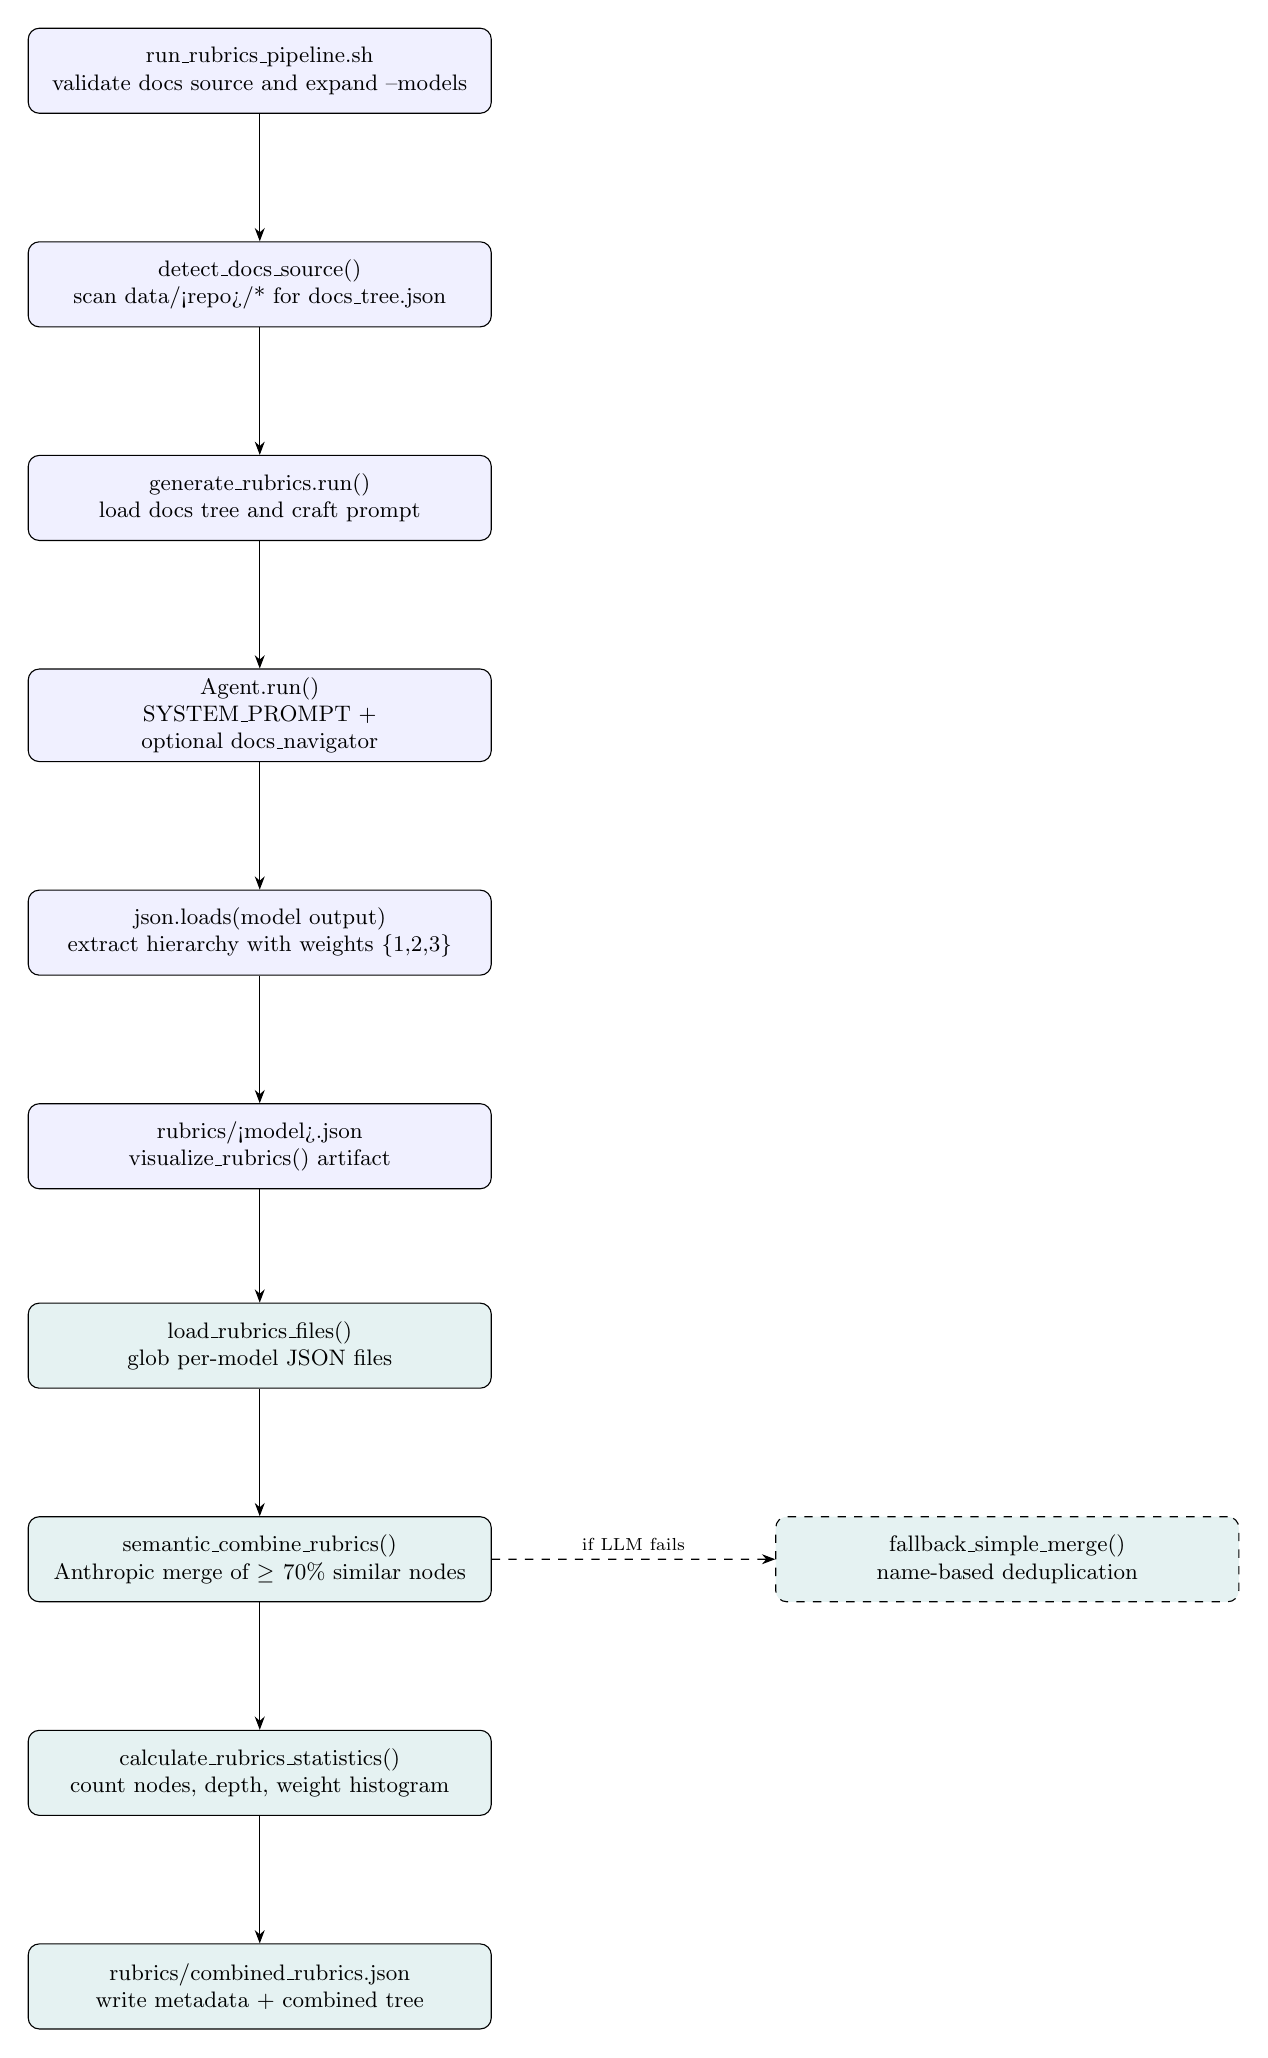
\begin{tikzpicture}[scale=0.9, transform shape, >=Stealth,
        node distance=1.8cm,
        stage/.style={draw, rounded corners, align=center, font=\small, text width=6.3cm, minimum height=1.2cm, fill=blue!6},
        comb/.style={draw, rounded corners, align=center, font=\small, text width=6.3cm, minimum height=1.2cm, fill=teal!10}]
        \node[stage] (P0) {run\_rubrics\_pipeline.sh\\validate docs source and expand --models};
        \node[stage, below=of P0] (P1) {detect\_docs\_source()\\scan data/<repo>/* for docs\_tree.json};
        \node[stage, below=of P1] (P2) {generate\_rubrics.run()\\load docs tree and craft prompt};
        \node[stage, below=of P2] (P3) {Agent.run()\\SYSTEM\_PROMPT + optional docs\_navigator};
        \node[stage, below=of P3] (P4) {json.loads(model output)\\extract hierarchy with weights \{1,2,3\}};
        \node[stage, below=of P4] (P5) {rubrics/<model>.json\\visualize\_rubrics() artifact};

        \node[comb, below=1.6cm of P5] (C0) {load\_rubrics\_files()\\glob per-model JSON files};
        \node[comb, below=of C0] (C1) {semantic\_combine\_rubrics()\\Anthropic merge of \(\geq 70\%\) similar nodes};
        \node[comb, below=of C1] (C3) {calculate\_rubrics\_statistics()\\count nodes, depth, weight histogram};
        \node[comb, below=of C3] (C4) {rubrics/combined\_rubrics.json\\write metadata + combined tree};
        \node[comb, right=4cm of C1, dashed] (C2) {fallback\_simple\_merge()\\name-based deduplication};

        \draw[->] (P0) -- (P1);
        \draw[->] (P1) -- (P2);
        \draw[->] (P2) -- (P3);
        \draw[->] (P3) -- (P4);
        \draw[->] (P4) -- (P5);
        \draw[->] (P5) -- (C0);
        \draw[->] (C0) -- (C1);
        \draw[->] (C1) -- (C3);
        \draw[->] (C3) -- (C4);
        \draw[->, dashed] (C1) -- node[above, font=\scriptsize]{if LLM fails} (C2);
    \end{tikzpicture}
    \caption{Rubric generation and combination pipeline}
\end{figure}

\section{Evaluation Pipeline}
The evaluation entry point mirrors the generation flow:
\begin{enumerate}
    \item Choose a reference docs folder via \texttt{--reference} (auto-detected when omitted).
    \item Load \texttt{rubrics/combined\_rubrics.json} (or a per-model file supplied via \texttt{--rubrics-file}).
    \item Collect leaf requirements and evaluate them with \texttt{judge/judge.py}. Each leaf gets a binary score and evidence.
    \item Propagate scores upward via \texttt{calculate\_scores\_bottom\_up}: every parent score is a weight-normalized sum of its children's scores.
    \item Combine multi-model evaluations through \texttt{combine\_evaluations.py} and optionally visualize the aggregated report.
\end{enumerate}

\begin{figure}[ht]
    \centering
    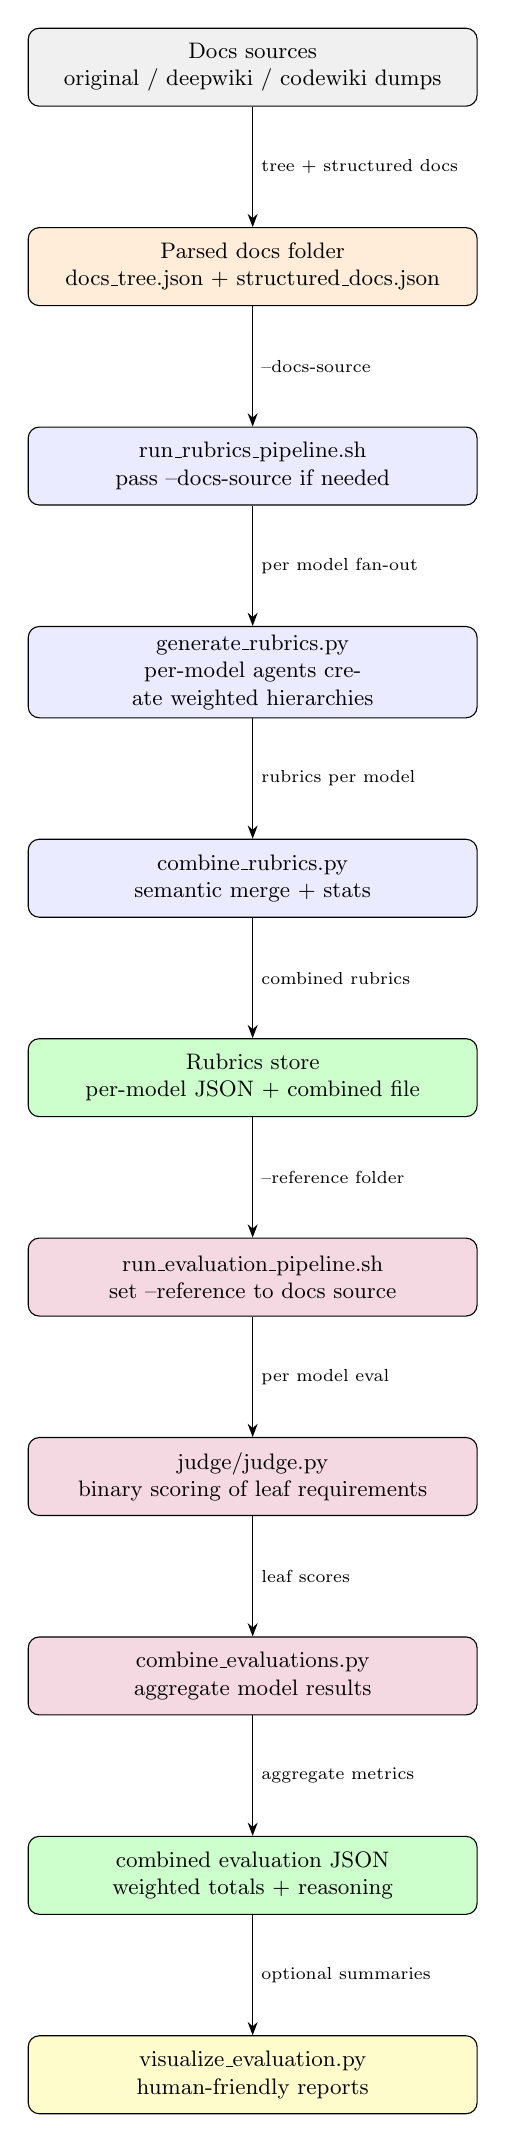
\begin{tikzpicture}[scale=0.9, transform shape, >=Stealth,
        node distance=1.7cm,
        stage/.style={draw, rounded corners, align=center, font=\small, text width=6.1cm, minimum height=1.1cm, fill=gray!12}]
        \node[stage] (S) {Docs sources\\original / deepwiki / codewiki dumps};
        \node[stage, below=of S, fill=orange!15] (P) {Parsed docs folder\\docs\_tree.json + structured\_docs.json};
        \node[stage, below=of P, fill=blue!8] (R) {run\_rubrics\_pipeline.sh\\pass --docs-source if needed};
        \node[stage, below=of R, fill=blue!8] (G) {generate\_rubrics.py\\per-model agents create weighted hierarchies};
        \node[stage, below=of G, fill=blue!8] (RC) {combine\_rubrics.py\\semantic merge + stats};
        \node[stage, below=of RC, fill=green!20] (RUB) {Rubrics store\\per-model JSON + combined file};
        \node[stage, below=of RUB, fill=purple!15] (E) {run\_evaluation\_pipeline.sh\\set --reference to docs source};
        \node[stage, below=of E, fill=purple!15] (J) {judge/judge.py\\binary scoring of leaf requirements};
        \node[stage, below=of J, fill=purple!15] (CE) {combine\_evaluations.py\\aggregate model results};
        \node[stage, below=of CE, fill=green!20] (COMB) {combined evaluation JSON\\weighted totals + reasoning};
        \node[stage, below=of COMB, fill=yellow!20] (VIS) {visualize\_evaluation.py\\human-friendly reports};

        \draw[->] (S) -- node[right, font=\scriptsize]{tree + structured docs} (P);
        \draw[->] (P) -- node[right, font=\scriptsize]{--docs-source} (R);
        \draw[->] (R) -- node[right, font=\scriptsize]{per model fan-out} (G);
        \draw[->] (G) -- node[right, font=\scriptsize]{rubrics per model} (RC);
        \draw[->] (RC) -- node[right, font=\scriptsize]{combined rubrics} (RUB);
        \draw[->] (RUB) -- node[right, font=\scriptsize]{--reference folder} (E);
        \draw[->] (E) -- node[right, font=\scriptsize]{per model eval} (J);
        \draw[->] (J) -- node[right, font=\scriptsize]{leaf scores} (CE);
        \draw[->] (CE) -- node[right, font=\scriptsize]{aggregate metrics} (COMB);
        \draw[->] (COMB) -- node[right, font=\scriptsize]{optional summaries} (VIS);
    \end{tikzpicture}
    \caption{Documentation, rubrics, and evaluation data flow}
\end{figure}

\section{End-to-End Algorithms}
Both pipeline orchestrations follow the same high-level pattern described in Issue \texttt{2025-11-18-12-20-22}: locate a parsed documentation folder, fan out per model, and persist JSON artifacts before any visualization or aggregation happens.

\subsection{Rubrics Pipeline Algorithm}
\begin{enumerate}
    \item \textbf{Docs source detection.} \texttt{run\_rubrics\_pipeline.sh} scans \texttt{data/\textless repo\textgreater/\*} for a folder that exposes \texttt{docs\_tree.json}. Operators can override the auto-detected folder via \texttt{--docs-source} to target \texttt{codewiki}, \texttt{deepwiki}, or any other parsed drop when \texttt{original/} is missing.
    \item \textbf{Model fan-out.} Once the source folder is confirmed, the script loops over the requested models (via \texttt{--models}) and calls \texttt{rubrics\_generator/generate\_rubrics.py} per model so that failures are isolated.
    \item \textbf{Agent execution.} The generator loads \texttt{docs\_tree.json}, optionally wires in the \texttt{docs\_navigator} tool, and asks the Pydantic-AI agent to return a weighted hierarchy with embedded documentation references.
    \item \textbf{Persistence and visualization.} Each output is saved to \texttt{rubrics/\textless model\textgreater.json}, after which \texttt{combine\_rubrics.py} may run to build \texttt{combined\_rubrics.json}, collect statistics (counts, depth, weight histogram), and optionally render a visual summary.
\end{enumerate}

\subsection{Evaluation Pipeline Algorithm}
\begin{enumerate}
    \item \textbf{Reference folder selection.} \texttt{run\_evaluation\_pipeline.sh} mirrors the earlier detection logic but reads \texttt{--reference} (default \texttt{original}). Any folder that exposes \texttt{docs\_tree.json} + \texttt{structured\_docs.json} can be supplied here.
    \item \textbf{Leaf scoring.} For each model, \texttt{judge/judge.py} loads the rubrics (combined or per-model), extracts every leaf requirement, and queries the model for a binary score with reasoning/evidence.
    \item \textbf{Score propagation and aggregation.} \texttt{calculate\_scores\_bottom\_up} normalizes each parent's score by the children's weights, \texttt{combine\_evaluations.py} fuses multi-model runs, and \texttt{visualize\_evaluation.py} can be used to export a narrative report.
\end{enumerate}

\subsection{Handling Missing \texttt{original/}}
Neither algorithm depends on the folder name; they only require the canonical parsed outputs. When \texttt{data/\textless repo\textgreater/original} is absent, run the rubrics pipeline with \texttt{--docs-source \textless existing\_folder\textgreater} and the evaluation pipeline with \texttt{--reference \textless existing\_folder\textgreater}. Both scripts abort early if \texttt{docs\_tree.json} is missing, which makes misconfigurations obvious.

\paragraph{Mermaid-style Summary.} The following block reproduces the execution sketch from the issue for quick embedding into README or wiki contexts:

\begin{verbatim}
```mermaid
flowchart TD
    S([Docs sources]) -->|tree + structured docs| P[Parsed folder]
    P -->|--docs-source| R[run_rubrics_pipeline.sh]
    R -->|per model| G[generate_rubrics.py]
    G --> RC[combine_rubrics.py]
    RC --> RUB[rubrics store]
    RUB -->|--reference| E[run_evaluation_pipeline.sh]
    E --> J[judge/judge.py]
    J --> CE[combine_evaluations.py]
    CE --> COMB[combined evaluation JSON]
    COMB --> VIS[visualize_evaluation.py]
```
\end{verbatim}

\end{document}
